%\title{Article HW Template}

\documentclass[12pt]{article}
\usepackage{ucs}
\usepackage[utf8x]{inputenc}
\usepackage[greek,english]{babel}
\newcommand{\en}{\selectlanguage{english}}
\newcommand{\gr}{\selectlanguage{greek}}

\usepackage[paper=a4paper,top=1in, bottom=1in, right=1in, left=.7in]{geometry}


\usepackage{amsthm, amssymb, amsfonts, amsmath}
\usepackage{graphicx}
\usepackage{tikz}
\usetikzlibrary{calc,shapes}
\usepackage{enumitem}
\usepackage{mathtools}
\usepackage{mathrsfs}
\usepackage{tikz-cd}
\usepackage{hyperref, mathabx}
\usepackage{algorithm}
\usepackage{algpseudocode}
\renewcommand{\algorithmicrequire}{\textbf{Input:}}
\renewcommand{\algorithmicensure}{\textbf{Output:}}


\newcommand{\boxitem}[2]{\vspace{.55cm}
	\item[#1]
	\leavevmode
	\strut
	\vadjust{%%
		\noindent
		\raisebox{\dimexpr\dp\strutbox+\ht\strutbox+1ex}[0pt][0pt]{\tikzmark{bl}}}%%
	#2
	
	\leavevmode
	\vadjust{%
		\noindent
		\hspace*{\dimexpr\textwidth+1ex}\tikzmark{br}}%%
	
	\tikz[overlay,remember picture]{\draw[black]
		(bl) rectangle
		(br);}}

\newcommand{\tikzmark}[1]{\tikz[overlay,remember picture] \node (#1) {};}

\newcommand{\R}{\mathbb{R}}
\newcommand{\Q}{\mathbb{Q}}
\newcommand{\Z}{\mathbb{Z}}
\newcommand{\N}{\mathbb{N}}
\newcommand{\p}{\mathbb{P}}
\newcommand{\E}{\mathbb{E}}
\newtheorem*{lemma}{Lemma}
\newtheorem{llemma}{Lemma}
\newtheorem*{theorem}{Theorem}
\newtheorem*{prop}{Proposition}

\begin{document}
	\null\hfill\begin{tabular}[t]{r@{}}
		Nikolas Mavrogeneiadis - 161014\\
		gravitorious \\
		University Of West Attica \\
		Department of Informatics and Computer Engineering\\
		Professor: Panagiotis Rouvelas\\
		\today
	\end{tabular}
	\\
	\centerline{\scshape{Graph Theory-Exercise Set 3}}
	
	\begin{enumerate}[listparindent=1.5em,
		parsep = 0pt]
		
		\boxitem{1.}{
			(From Set 2 exercise 4)Let G be a simple graph. Prove that if $L(G)$ is Eulerian, then we can't conclude that G is Eulerian.
		}
		\underline{Proof:} 
		If $L(G)$ is Eulerian this means that each vertex degree of $L(G)$ is even number. This vertex will become an edge $e(v,u)$ on $G$ with $deg(v)+deg(u) = even$. In this case, we can't deduce whether $deg(v)$ and $deg(u)$ are even or not. The line graph of $K_{4}$ (on the right in the following picture) is Eulerian but the $K_4$ is not Eulerian itself (all vertices have odd degree as we can see on the left).
		This completes the proof.
		\begin{figure}[h]
			\centering
			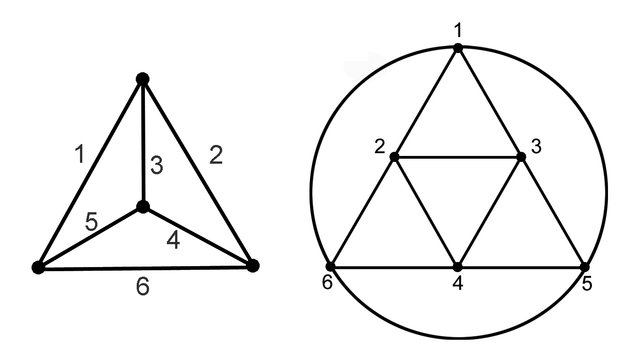
\includegraphics[width=0.55\textwidth]{ex1}
			\caption{$K_{4}$ and its Line graph}
			\label{fig:mesh1}
		\end{figure}\\
	
		\boxitem{2.}{
			\gr (Ασκηση 5 από το σετ 2)Δείξτε ότι αν ένας γράφος με τουλάχιστον 3 κορυφές που έχει απομονωμένη ή εκκρεμή κορυφή, τότε έχει μη πλήρη κλειστότητα.
		}
		Εστω μια κορυφή $v_{k}$ με $d(v_{k})\leq1$. Εστω $v_{i}$ ο προς εξέταση κόμβος για το αν θα υπάρξει ακμή $e(v_{k}, v_{i})$ στην κλειστότητα του γράφου. Προφανώς ο $v_{k}$ δεν είναι γείτονας με τον $v_{i}$ στον αρχικό γράφο. Για να υπάρξει ακμή θα πρέπει $d(v_{i}) + d(v_{k})\geq n$, δηλαδή $d(v_{i})\geq n-1$. Αυτό όμως είναι αδύνατον γιατί αν ίσχυε ότι $d(v_{i}) = n-1$ τότε οι δύο κόμβοι θα ήταν γειτονικοί στον αρχικό κόμβο, πράγμα άτοπο. Επομένως αυτοί οι δύο κόμβοι δεν θα γίνουν γειτονικοί στην κλειστότητα και άρα η κλειστότητα δεν είναι πλήρης.

		\newpage

		\boxitem{3.}{
			(Ασκηση 8 από το σετ 2) Δείξτε ότι αν ένας διμερής γράφος είναι περιττής τάξης, τότε δεν είναι Hamiltonian.
		}
		Εστω ο διμερής γράφος $K(n,m)$ για τον οποίο ισχύει ότι $n+m=odd$. Χωρίς βλάβη της γενικότητας υποθέτουμε ότι $n>m$. Θέτουμε $S_{1} = \{v_{11}, v_{12}, ..., v_{1n}\}$ το σύνολο με τις $n$ κορυφές και $S_{2} = \{v_{21}, v_{22}, ..., v_{2m}\}$ το σύνολο με τις $m$ κορυφές του $K$. Αν υπάρχει \en Hamiltonian \gr κύκλος, τότε αυτό θα πρέπει να περιέχει όλους τους κόμβους του $S_{1}$. Εστω ο $v_{1k}$ και ο $v_{1p}$ ο πρώτος και ο τελευταίος κόμβος που επισκεπτόματε από το $S_{1}$ με την προυπόθεση ότι έχουμε επισκεφθεί όλους τους κόμβους του. Το μονοπάτι αυτό είναι της μορφής $H=\{ v_{1k}, ..., v_{1p}\}$. Ομως για κάθε ζευγάρι κόμβων $(v_{1i}, v_{1(i+1)})$ του $S_{1}$ πρέπει αναγκαστικά να επισκεφθούμε έναν κόμβο του $S_{2}$. Αυτό σημαίνει ότι το $H$ περιλαμβάνει και όλους τους κόμβους του $S_{2}$ (αφού $n>m$). Για να είναι το $H$ \en Hamiltonian \gr κύκλος θα πρέπει ο $v_{1p}$ να συνδέεται με τον $v_{1k}$ κάτι το οποίο είναι αδύνατον αφού ο $v_{1p}$ συνδέεται μόνο με κόμβους του $S_{2}$ που ήδη τους έχουμε επισκεφτεί. Επομένως ο γράφος δεν είναι \en Hamiltonian.
		
		\gr
		\boxitem{4.}{
			(Ασκηση 1 από το σετ 3 - όλες οι παρακάτω ασκήσεις αφορούν το σετ 3)Δείξτε ότι κάθε δέντρο είναι διμερής γράφος.
		}
		Εστω δύο σύνολα $X$ και $Y$ τα οποία κατασκευάζουμε ως εξής. Επιλέγουμε από το δέντρο μια ρίζα. Τοποθετούμε στο $X$ την ρίζα και όλες τις κορυφές που απέχουν από αυτή απόσταση ίση με άρτιο αριθμό. Στο $Y$ τοποθετούμε όσες κορυφές απέχουν απόσταση ίση με περιττό αριθμό. Θα δείξουμε ότι δεν υπάρχουν κορυφές που ενώνονται μεταξύ τους στο $X$, ούτε στο $Y$ και άρα ο γράφος είναι διμερής. Εστω δύο κόμβοι $x_{1}$ και $x_{2}$ του $X$ και έστω ότι ενώνονται. Εστω $x_{0}$ η ρίζα του δέντρου. Τότε μπορούμε να κατασκευάσουμε το μονοπάτι $\{x_{0}, ... ,x_{1}, x_{2}, ..., x_{0}\}$ το οποίο είναι κύκλος. Ατοπο. Παρόμοια μπορούμε να το δείξουμε και για το $Y$.
		
		\boxitem{4.}{
			(Ασκηση 2) Δείξτε ότι κάθε δέντρο $T$ έχει τουλάχιστον $D(T)$ εκκρεμείς κορυφές.
		}
		Εστω ότι υπάρχει δέντρο $T$ με $p$ εκκρεμείς κορυφές και ισχύει ότι $p < D(T)$. Επιλέγω μια ρίζα $k$ για την οποία ισχύει ότι $d(k) = D(T)$. Εστω το σύνολο $X=\{v_{1}, v_{2}, ..., v_{D(T)}\}$ που περιέχει τους γείτονες του $k$. Κάθε εκκρεμής κορυφή έχει μοναδικό μονοπάτι ως προς τον $k$, όπου αναγκαστικά πρέπει να περάσει από κάποιο κόμβο του $X$. Ο κόμβος από τον οποίο μπορεί να περάσει είναι μοναδικός (αλλιώς θα υπήρχε κύκλος). Ομως επειδή οι εκκρεμείς κορυφές είναι λιγότερες από $D(T)$, υπάρχει κορυφή $v_{i}$ του $X$ που δεν χρησιμοποιείται ποτέ από μονοπάτι εκκρεμούς κορυφής ως προς τον $k$. Αυτό όμως σημαίνει ότι και η $v_{i}$ είναι εκκρεμής κορυφή. Ατοπο.

		\newpage

		\boxitem{5.}{
			(Ασκηση 3) Δείξτε ότι κάθε δένδρο χωρίς κορυφές βαθμού 2 έχει περισσότερες εκκρεμείς απ'ό,τι μη εκκρεμείς κορυφές.
		}
		Εστω $k$ ο αριθμός των φύλλων (εκκρεμείς κορυφές) και $p$ οι υπόλοιπες κορυφές. Γνωρίζουμε ότι $|E| = |V| - 1$. Είναι:
		\begin{equation}
			 \sum_{v \in V}^{}d(v) = 2|E| = 2|V| - 2
		\end{equation}
		Εστω τα σύνολα $F=\{f_{1}, f_{2}, ..., f_{k}\}$ και $V=\{v_{1}, v_{2}, ..., v_{p}\}$. 
		\\
		Είναι:
		\begin{equation}
			\begin{split}
				 2|V| - 2 &= \sum_{i=1}^{k}d(f_{i}) +  \sum_{j=1}^{p}d(v_{j}) \\ 
						&\geq k + 3p
			\end{split}
		\end{equation}
		Αρα μπορούμε να γράψουμε ότι:
		\begin{equation}
			\begin{split}
				 &2|V| - 2 \geq k + 3p \\
				  \Longrightarrow &2k + 2p - 2 \geq k + 3p \\
				  \Longrightarrow &k-p-2 \geq 0 \\
				  \Longrightarrow &k \geq p + 2 \\
				  \Longrightarrow &k \geq p
			\end{split}
		\end{equation}
		
		\boxitem{5.}{
			(Ασκηση 4) Εστω $T=(V,E)$ δένδρο και $f:T\longrightarrow T$ ισομορφισμός τέτοιος ώστε για κάθε $v\in V, f(v) \neq v$. Δείξτε ότι υπάρχουν $u,v\in V$ έτσι ώστε $(u,v)\in E$, $f(u)=v$ και $f(v)=u$.
		}

		Αρχικά ο ισομορφισμός θα πρέπει να κάνει $map$ κάθε φύλλο του δέντρου σε κάποιο (διαφορετικό) φύλλο του δέντρου. Εστω το δέντρο $T_{2}$ που προέρχεται από το $T$ χωρίς τα φύλλα του $T$. Είναι προφανές ότι ο ίδιος ισομορφισμός που χρησιμοποιήσαμε για το αρχικό δέντρο, ισχύει και για το $T_{2}$ γιατί αν δεν ίσχυε, τότε αυτό θα σήμαινε ότι κάποιος κόμβος του $T$ που δεν είναι φύλλο, κάνει $map$ σε κορυφή που είναι φύλλο, κάτι που δεν γίνεται. Εστω ότι επαναλαμβάνουμε την διαδικασία μέχρι να μείνουν 1 ή 2 κορυφές (δηλαδή 1 κορυφή μόνη της ή 2 κορυφές με μια ακμή). Ομως αν έχει μείνει μόνο 1 κορυφή δεν γίνεται να ισχύει ο ισομορφισμός από υπόθεση. Αναγκαστικά λοιπόν θα έχουν μείνει 2 κορυφές με 1 ακμή και αφού ο ισομορφισμός ισχύει για κάθε δέντρο $T_{i}$, τότε θα πρέπει η κάθε μια από τις 2 κορυφές να κάνει $map$ στην άλλη (δεν γίνεται η κάθε κορυφή να κάνει $map$ στον εαυτό της από υπόθεση). Αρα το συμπέρασμα ισχύει.

		\newpage

		\boxitem{6.}{ (Ασκηση 5)
			$(i)$ Βρείτε το δέντρο που αντιστοιχεί στην ακολουθία $Prufer$ $(7,7,1,3,4)$. \\
			$(ii)$ Βρείτε το δέντρο που αντιστοιχεί στην ακολουθία $Prufer$ $(i,i,...,i)$ μήκους $n-2$, όπου $1 \leq i < n$ και $n > 2$. \\
			$(iii)$ Βρείτε την ακολουθία $Prufer$ του εξής δέντρου:
			\begin{figure}[h]
				\centering
				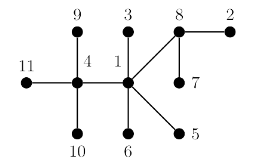
\includegraphics[width=0.30\textwidth]{pic1}
				\caption{}
				\label{fig:mesh1}
			\end{figure}
		}
		
		$(i)$  \\
		\begin{figure}[h]
				\centering
				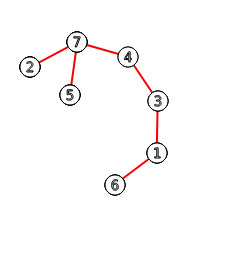
\includegraphics[width=0.30\textwidth]{pic2}
				\caption{Δέντρο ακολουθίας $Prufer$ $(7,7,1,3,4)$}
				\label{fig:mesh1}
		\end{figure}

		$(ii)$  \\
		\begin{figure}[h]
				\centering
				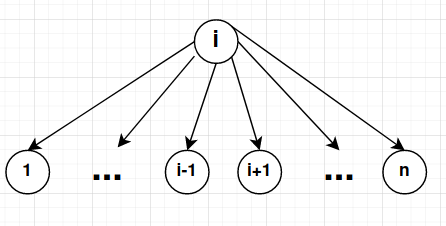
\includegraphics[width=0.45\textwidth]{pic3}
				\caption{Δέντρο ακολουθίας $Prufer$ $(i, i, ..., i)$}
				\label{fig:mesh1}
		\end{figure}
		\\	
		Προφανώς αν $i=1$ τότε το πρώτο φύλλο του δέντρου είναι το $i+1$.
		
		\newpage
		$(iii)$  
			
		Η ακολουθία είναι: (8,1,1,1,8,1,4,4,4).
		
		\boxitem{7.}{
			(Ασκηση 6) Πόσα ζευγνύοντα δέντρα του $K_{n}$ έχουν ως φύλλο (δηλαδή εκκρεμή κορυφή) μια συγκεκριμένη κορυφή;
		}
		Εστω ο γράφος $Κ_{n}$ και μια $v$ μια συγκεκριμένη κορυφή του. Ο γράφος $K_{n}-v$ είναι προφανές ο $K_{n-1}$. Ο αριθμός των ζευγνύοντων δέντρων του $K_{n-1}$ είναι $(n-1)^{n-3}$. Προσθέτοντας τώρα την κορυφή $v$ σε κάθε ζευγνύον δέντρο, έχουμε $n-1$ επιλογές σε κάθε ένα από αυτά. Συνολικά λοιπόν ο αριθμός των ζευγνύοντων δέντρων του $K_{n}$ με σταθερή μια συγκεκριμένη κορυφή είναι $(n-1)^{n-3} * (n-1)$ = $(n-1)^{n-2}$.
		
		\boxitem{8.}{
			(Ασκηση 7) Μπορούν οι αλγόριθμοι του $Prim$ και του $Kruskal$ να εφαρμοστούν σε ζυγισμένους γράφους με αρνητικά βάρη;
		}
 		Και οι δύο αλγόριθμοι μπορούν να εφαρμοστούν σε αλγόριθμους με αρνητικά βάρη. Στον αλγόριθμο του $Krustal$ η επόμενη ακμή με το χαμηλότερο βάρος που θα προσθέσουμε μπορεί να είναι αρνητική. Αυτό δεν αλλάζει το πως δουλεύει ο αλγόριθμος γιατί και πάλι θα επιλέγει πάντα την ακμή με το χαμηλότερο βάρος και το συνολικό βάρος του παραγόμενου ζευγνύον δέντρου θα είναι ο μικρότερος δυνατός. Παρόμοια ισχύει και για τον αλγόριθμο του $Prim$.
		
		\boxitem{9.}{
			(Ασκηση 8) Ορίστε αλγόριθμο που δέχεται ως είσοδο έναν συνδεδεμένο γράφο και μια ακμή του και επιστρέφει το ελάχιστο ζευγνύον δέντρο του γράφου αυτού που περιέχει τη συγκεκριμένη ακμή.
		}
		
		Εστω ότι εφαρμόζουμε τον αλγόριθμο του $Krustal$ στον συνδεδεμένο γράφο. Ως αποτέλεσμα θα πάρουμε το ελάχιστο ζευγνύον δέντρο $Τ$. Αν αυτό το $Τ$ περιέχει την ακμή που θέλουμε τότε δεν χρειάζεται να κάνουμε κάτι άλλο. Εστω ότι δεν την περιέχει. Τότε προσθέτουμε την ακμή αυτή στο $T$. Τότε δημιουργείται ένας κύκλος. Ελέγχουμε κάθε ακμή σε αυτόν τον κύκλο (εκτός από αυτή που προσθέσαμε) ώστε να δούμε αν υπάρχει ακμή με το ίδιο βάρος με την ακμή που προσθέσαμε. Αν υπάρχει, τότε την αφαιρούμε και το νέο $Τ$ είναι το ζητούμενο δέντρο. Αν δεν υπάρχει τέτοια ακμή, τότε δεν υπάρχει ελάχιστο ζευγνύον δέντρο με αυτή την ακμή.
		


	\end{enumerate}
\end{document}
